\speciestitle{Hydrogen Cyanide}{HCN}{HCN}{%
  \item[Useful range:] 68--32\,hPa (use with caution) 21--0.1\,hPa (no restrictions)
  \item[Product lead:] Hugh C. Pumphrey
  \item[Contact:] Luis Mill\'an,
 \email{Luis.F.Millan@jpl.nasa.gov}}

\subsection{Introduction}

MLS observes \ch{HCN} emission lines within the 190-GHz radiometer. The spectral signature
of \ch{HCN} in the MLS radiances is weak, a relatively strong smoothing constraint is required to obtain meaningful retrievals, and averaging (e.g., weekly zonal means) is recommended.

Table \ref{tab:HCNSummary} summarizes the precision, accuracy, and resolution of the MLS \ch{HCN} product. The MLS \thisv \ch{HCN} data are scientifically useful over the range 21
to 0.1\,hPa. At 68–32,hPa, the data may still be usable with caution for qualitative studies. More details on details on the \ch{HCN} measurement, may be found in \cite{PumphreyEtal:2006}.

% HCN is retrieved from bands encompassing, in the lower sideband, the 177.26\,GHz spectral line of HCN\@. Although the target line is in an uncluttered part of the spectrum, the upper sideband contains many interfering lines of \ch{O3} and \ch{HNO3}. As a result, the \thisv HCN product is not recommended for general use at altitudes below 21\,hPa. In the recommended range it is usable but has rather poor precision (necessitating averaging such as weekly zonal means) and resolution.

% It is possible to retrieve weekly zonal means of HCN over a greater vertical range by first averaging the radiances. Results of this process and further information on the HCN measurement may be found in \cite{PumphreyEtal:2006}. 

\subsection{Differences between earlier versions and \thisv}

No changes specific to the HCN retrieval were made between \vii and \viii. For \viv, a new phase was introduced in which HCN is retrieved using only Bands 6 and 27, rather than all of R2; this phase is also used in \thisv. The \viv HCN had obvious biases in the lower stratosphere, but they were far less severe than in \vii and \viii, both of which had large regions with negative mixing ratios. In \prevv and \thisv the biases appear to be reduced further; the changes between \prevv and \thisv are small. Between 10 and 3\,hPa, \prevv and \thisv HCN are somewhat lower than all prior versions. 

%The lowest recommended level for \thisv is currently 21\,hPa, as it was for \prevv and \viv. 

%However, it is possible that further validation work could show that the \thisv HCN data are suitable for scientific use between 31\,hPa and 68\,hPa.

Figure~\ref{fig:HCNPrecision} shows that the precisions in \thisv are essentially unchanged from earlier versions. The retrieved mixing ratios change very little in the region where use was recommended for earlier versions. Mixing ratios are considerably different between all five earlier versions in the lower stratosphere. However, the profile shape in \thisv appears less unrealistic than in any prior version.

\subsection{Vertical resolution}
\onestandardavk{HCN}{HCN}%

The HCN signal is fairly small, so a rather strong smoothing constraint has to be applied to ensure that the retrieval is at all useful. As Figure~\ref{fig:AvkHCN} shows, the vertical resolution is about 8\,km at 10\,hPa, degrading to more than 12\,km at 0.1\,hPa. The horizontal resolution along the measurement track is between 2 and 4 profile spacings.

\subsection{Precision}

Figure~\ref{fig:HCNPrecision} shows the estimated precision (values of the field \texttt{L2gpPrecision}), together with the observed standard deviation in an equatorial latitude band where the natural variability of the atmosphere is small. The observed scatter is smaller than the estimated precision due to the effects of retrieval smoothing.

% \begin{figure}
%   \centering%
%   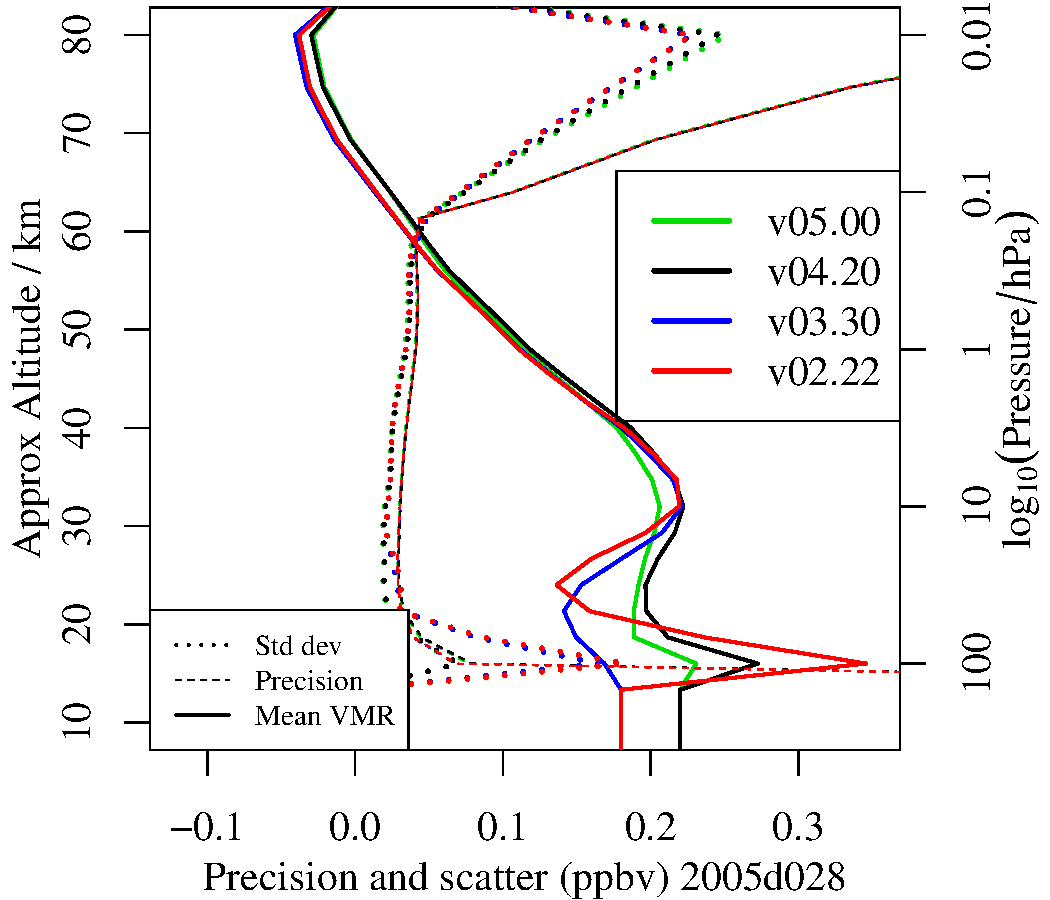
\includegraphics[width=0.495\textwidth]{figures/hcn-prec-fig-eq-2005d028}\hfill%
%   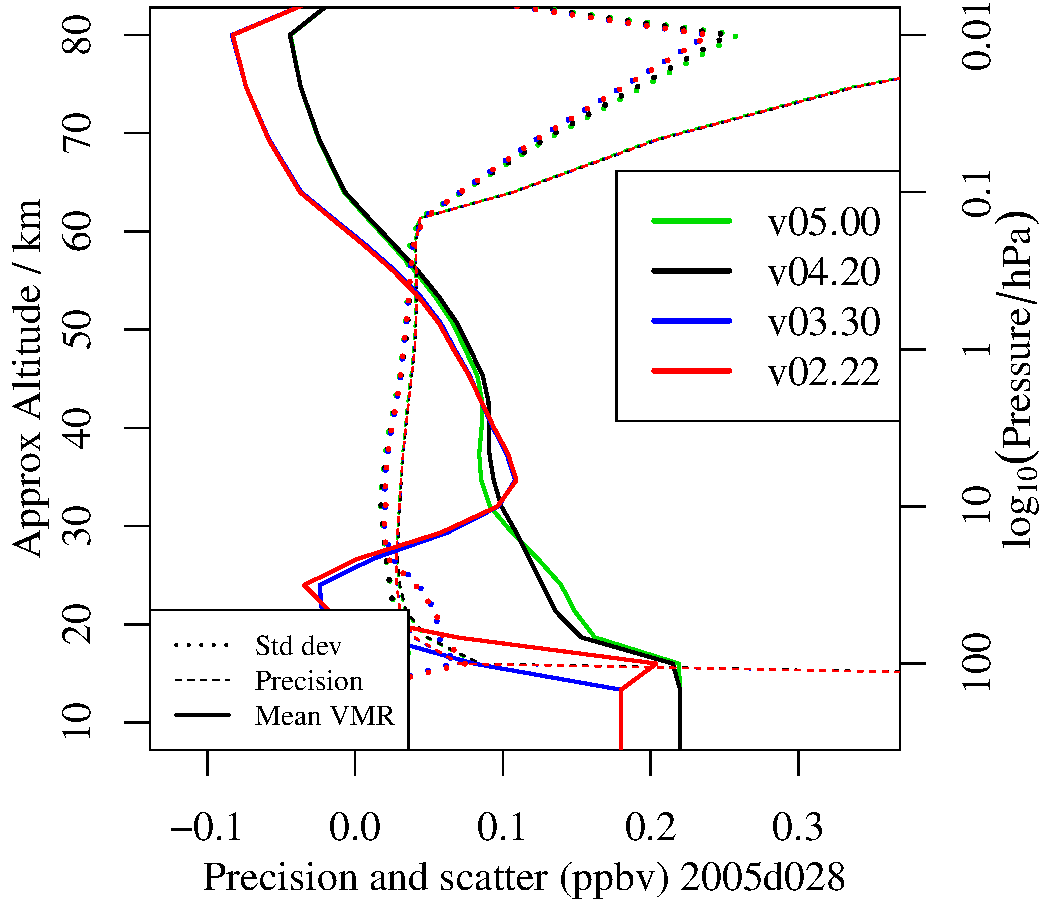
\includegraphics[width=0.495\textwidth]{figures/hcn-prec-fig-NP-2005d028}
%   \caption{Estimated precision {\tt L2gpPrecision} and observed standard deviation for MLS \thisv (orange), \prevv (green), v4.x (black), v3.x (blue) and v2.x (red) HCN\@. The data shown are all profiles within 20\degsym\ of the equator (left) and 70\degsym N--83\degsym N (right) for 28 January, 2005.  Mean mixing ratio (VMR) profiles are shown for comparison. Between 3 and 10\,hPa, \thisv and \prevv depart from the three earlier versions. At altitudes below 10\,hPa, all five versions are different, but v2.x and v3.x are less realistic than v4.x, \prevv, and \thisv.}
%   \label{fig:HCNPrecision}
% \end{figure}

\begin{figure}
  \centering%
  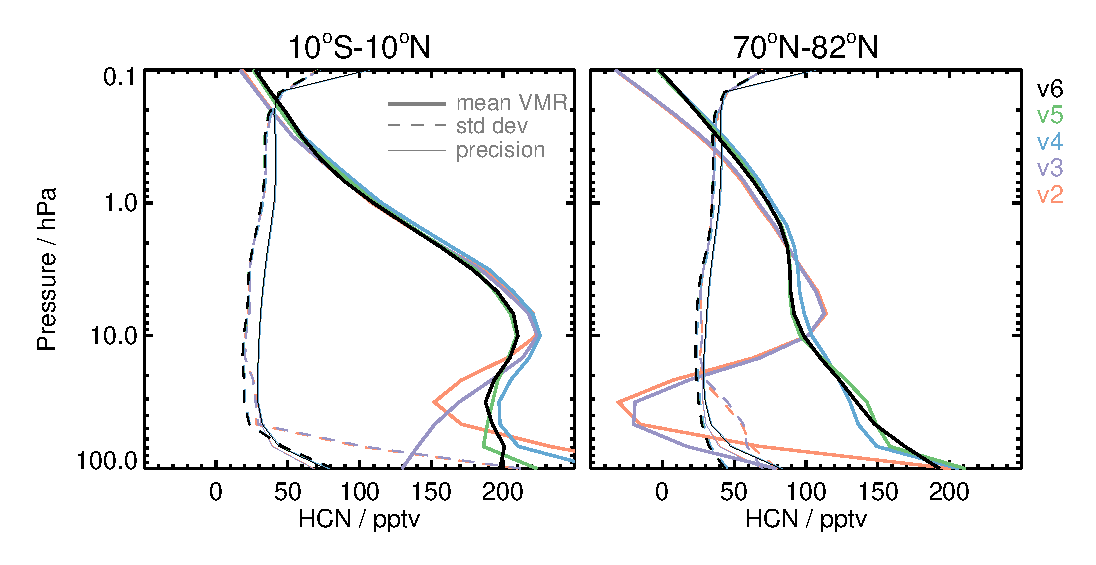
\includegraphics[width=0.9\textwidth]{figures/hcn_prof}
  \caption{Estimated precision {\tt L2gpPrecision} (thin lines) and observed standard deviation (dashed lines) for MLS \thisv (black), \prevv (green), v4.x (blue), v3.x (purple) and v2.x (red) HCN\@. The data shown are for the 10\degsym\,S to 10\degsym\,N (left) and 70\degsym\,N--82\degsym\,N (right) for 28 January, 2005.  Mean volume mixing ratio (VMR) profiles are shown for comparison. Between 3 and 10\,hPa, \thisv and \prevv depart from the three earlier versions. Below 10\,hPa, all five versions are different, but v2.x and v3.x are less realistic than v4.x, \prevv, and \thisv.}
  \label{fig:HCNPrecision}
\end{figure}


\subsection{Accuracy}

The accuracy of the HCN product has not been assessed in detail because a cursory inspection revealed that \vii and \viii HCN had extremely large systematic errors in the lower stratosphere. These errors are much smaller in \viv.  In \prevv and \thisv the errors are improved over those in \viv in some places and somewhat worse in others, while being far better than in earlier versions. Some comparisons with ACE-FTS data are shown in Figure~\ref{fig:HCNvsACE}. At 21\,hPa and higher altitudes the two instruments agree well, with MLS versions \prevv and \thisv agreeing better with ACE-FTS than \viv. In the tropics, the two instruments agree well in the 32--68\,hPa range apart from a constant systematic error. At middle and high latitudes, the MLS data differ considerably from ACE-FTS in a long-term (\mytexttilde10-year) average; the differences include a decrease at the lowest altitudes. However, the seasonal and interannual variability show many similarities between the two instruments. The MLS data in the lower stratosphere can therefore be used with caution; comparison with ACE-FTS data is advisable. In the upper stratosphere, the values are in line with current understanding of the chemistry of HCN\@. Comparison to historical values suggests an accuracy of no worse than 50\%. 

\begin{figure}
% 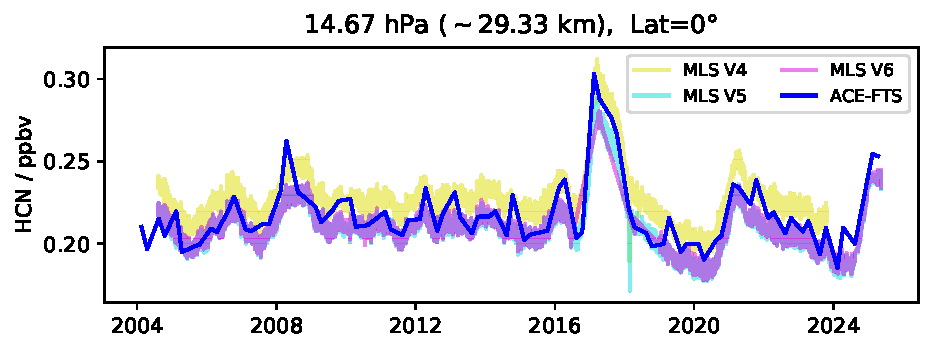
\includegraphics[width=0.82\textwidth]{figures/mls_ace_HCN_0_14-67.pdf}\\
% 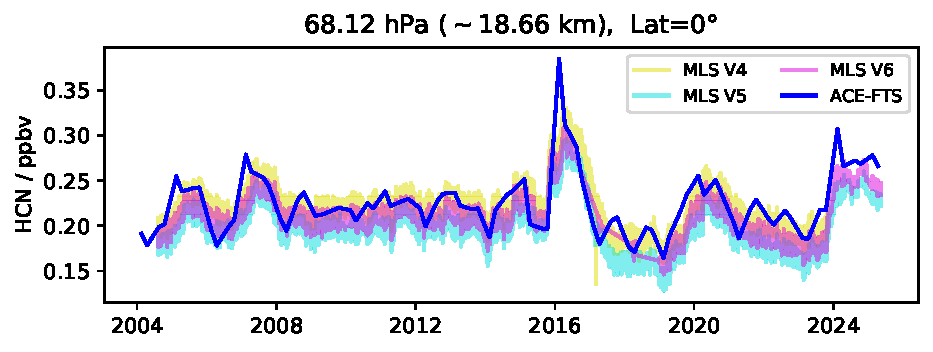
\includegraphics[width=0.82\textwidth]{figures/mls_ace_HCN_0_68-12.pdf}\\
% 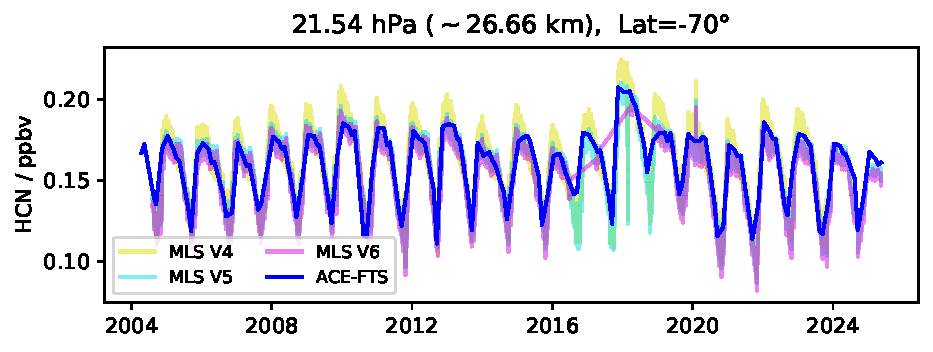
\includegraphics[width=0.82\textwidth]{figures/mls_ace_HCN_-70_21-54.pdf}\\
% 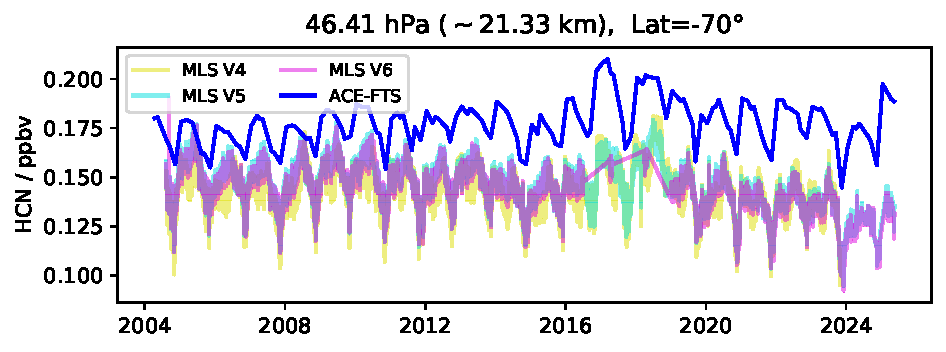
\includegraphics[width=0.82\textwidth]{figures/mls_ace_HCN_-70_46-41.pdf}
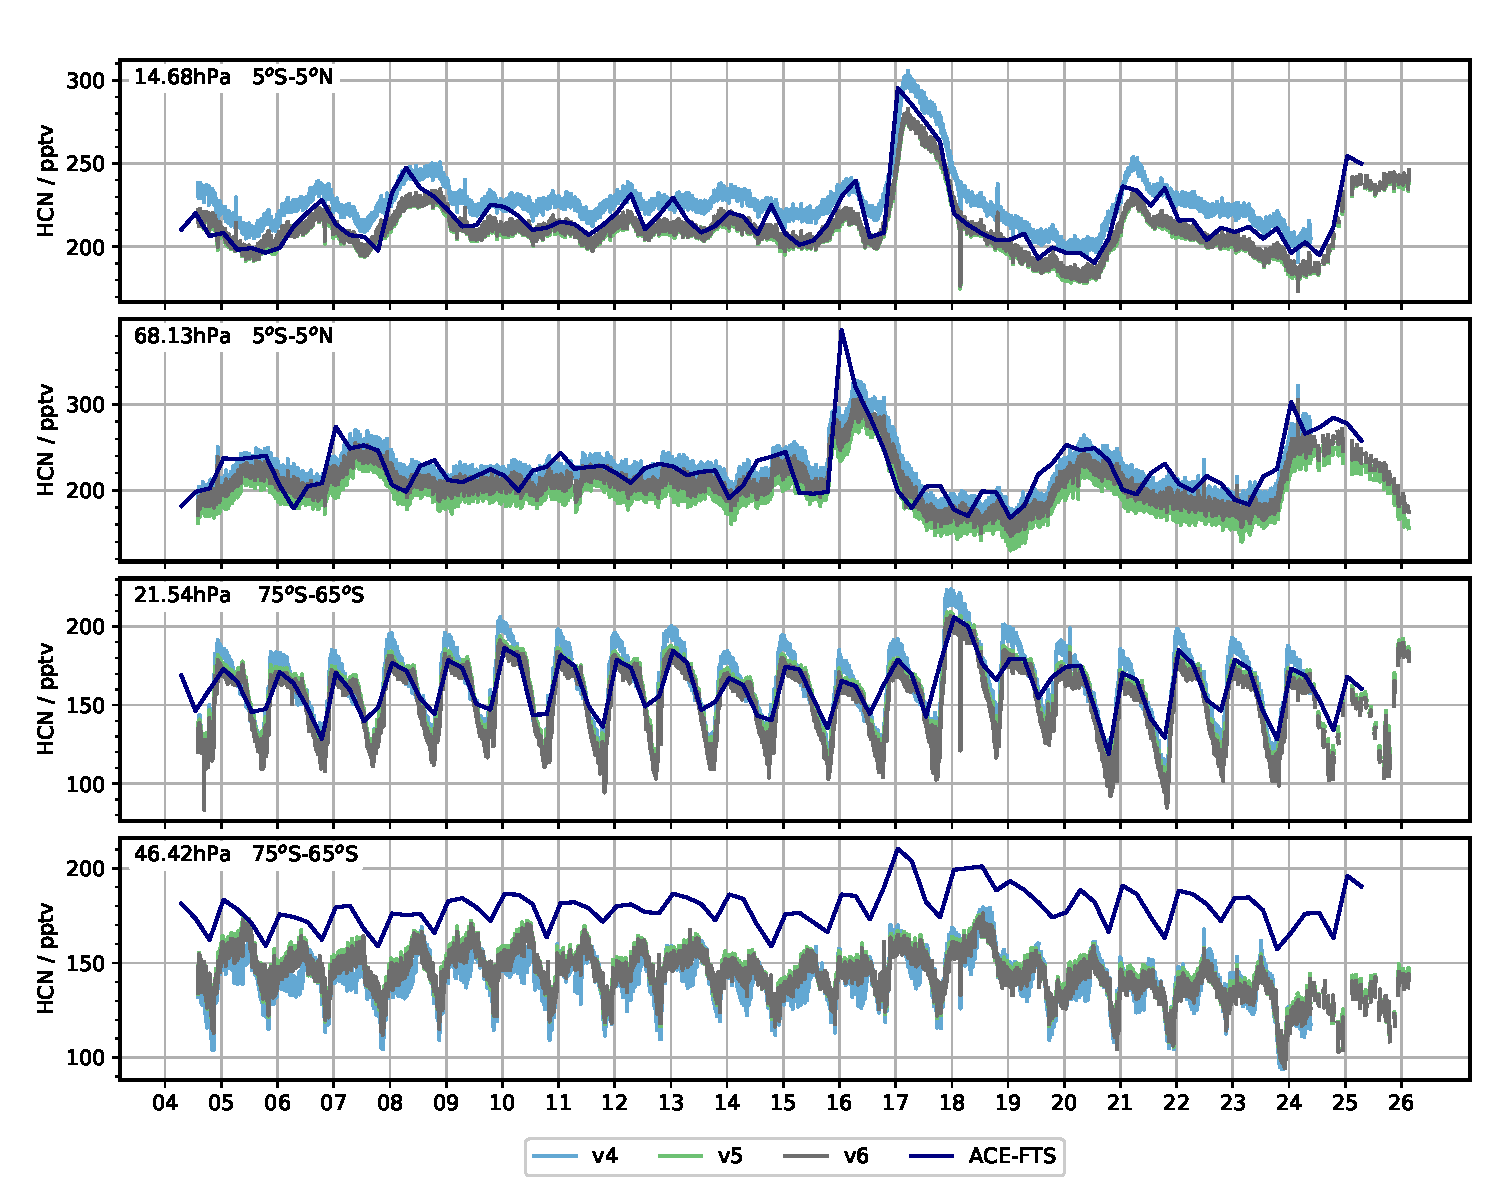
\includegraphics[width=0.9\textwidth]{figures/HCN_timeseries.pdf}
\caption{\label{fig:HCNvsACE} Daily time series of HCN at selected latitudes and pressure levels from MLS versions \viv, \prevv, and \thisv, with seasonal ACE-FTS version~5.3 for comparison.  }
\end{figure}

\begin{nofloatpages}
\subsection{Data screening}
\label{sec:HCNScreening}
\begin{description}
  \item[Pressure range:] \screeningrule{21--0.1\,hPa} \standardrangestatement\ Data in the 68\,hPa to 32\,hPa range may prove to be usable after further validation. \standardprecisionrule \evenstatusrule
  \item[Clouds:] \screeningrule{Clouds have no impact; profiles with non-zero even values of \texttt{Status} are suitable for use.} As HCN is only generally recommended in regions unaffected by clouds, profiles which have either, both, or neither of the cloud flags set may be used.
  \item[Quality:] \qualityrule{0.2} Values of \texttt{Quality} are usually near 1.5; occasional lower values do not seem correlated with unusual profiles, but we suggest as a precaution that only profiles with \texttt{Quality} $> 0.2$ be used. Typically this will eliminate only 1--2\% of profiles.
    %% Number of rejected profiles remains small in V5
  \item[Convergence:] \convergencerule{2.0} This should eliminate any chunks that have obviously failed to converge (typically only 1--2\% of the total).
    %% Number of rejected profiles remains small in V5
\end{description}
\end{nofloatpages}

\subsection{Artifacts}

There are no obvious artifacts within 21-0.1\,hPa recommended pressure range. At 68–32\,hPa, the data may be usable with caution for qualitative studies, and comparison with ACE-FTS measurements is recommended.

% \subsection{Desired improvements for future data version(s)}

% Hopefully it will prove possible to make further improvements to the retrieval of HCN in the lower stratosphere.

\begin{table}
% The precision and scatter are essentially identical in all of versions 4, 5 and 6, so this table is not changed from earlier versions of this document
  \caption{Summary of Aura MLS \thisv HCN Characteristics}
  \vspace{\tablecaptionsep}
  \label{tab:HCNSummary}
    \begin{minipage}{\linewidth}
    \renewcommand{\thefootnote}{\thempfootnote}
  \centering\begin{tabular}{ccccl}
  \toprule
  \parbox[m]{18mm}{\bfseries\centering Pressure\\ hPa} &
  \parbox[m]{22mm}{\bfseries\centering {Resolution\\ V $\times$ H%
  \footnote{Vertical and along-track horizontal resolutions; cross-track horizontal resolution is \mytexttilde9\,km.} \\ km}} &
  \parbox[m]{22mm}{\bfseries\centering Single-Profile\\ Precision%
  \footnote{The precision shown is the estimated precision (\texttt{L2gpPrecision}); the observed scatter is about 80\% of this value.} \\pptv} &
  \parbox[m]{20mm}{\bfseries\centering Accuracy \\ pptv} &
  \parbox[m]{40mm}{\bfseries Comments}\\
  \midrule
  $< 0.1$     & ---             &  --- &  ---      & Unsuitable for scientific use\\
  1--0.1      & 12 $\times$ 500 & 50   & 5         & \\
  21--1       & 10 $\times$ 300 & 40   & 15        & \\
  68--21      & 10 $\times$ 300 & 40   & 60        &  Use with caution\\
  100         & 10 $\times$ 300 & 50   & 130       &  Unsuitable for scientific use\\
  $> 100$     &                 &      &           &  Not Retrieved\\
  \bottomrule
\end{tabular}
\end{minipage}
\end{table}
